\chapter{Obtención, procesado y almacenamiento de los datos}


%Obtencion
Los datos provienen del artículo  Chemical gas sensor drift compensation using classifier ensembles \cite{GasData},

donde el objetivo era tratar de detectar el drift (la deriva) de los sensores a lo largo de los meses, y poder calibrarlos
utilizando el minimo numero de experimentos posibles. Es decir, de la forma más rápida y eficiente posible.
(ver \cite{GasData})

Los datos estan disponibles para su descarga desde
\href{https://archive.ics.uci.edu/ml//datasets/Gas+Sensor+Array+Drift+Dataset#}{UCI data repository}.
en 10 archivos formato \emph{.dat}.

Cada lote cuenta con una estructura de 129 columnas, donde la primera nos informa del gas y la concentración,
y el resto es la información obtenida del sensor.

El primer paso que se va a realizar es, dada las 128 componentes X,
averiguar a qué tipo de gas pertenece la medición.

Una vez la red es capaz de inferir correctamente de qué gas se trata,
alimentaremos otra red cuya función
sea averiguar la concentración del mismo.

\subsection{Procesado}

La lectura de los archivos  \emph{.dat} se ha realizado utilizando
el código adjunto en Apéndices  \ref{LoadUciData}


\subsection{Exploratory Data Analysis}

Los datos se nos presentan en 10 lotes, correspondientes a experimentos a lo largo de tres años, donde se ensayaron
6 diferentes gases a diferentes concentraciones.

\begin{table}[h!]
\begin{tabular}{|l|l|}
\hline
Batch ID & Month IDs                   \\ \hline
Batch 1  & Months 1 and 2              \\
Batch 2  & Months 3, 4, 8, 9 and 10    \\
Batch 3  & Months 11, 12, and 13       \\
Batch 4  & Months 14 and 15            \\
Batch 5  & Month 16                    \\
Batch 6  & Months 17, 18, 19, and 20   \\
Batch 7  & Month 21                    \\
Batch 8  & Months 22 and 23            \\
Batch 9  & Months 24 and 30            \\
Batch 10 & Month 36                    \\ \hline
\end{tabular}
    \caption{ Distribución de los lotes a lo largo del tiempo.}
\end{table}

Los gases que se estudiaron son los siguientes:
\begin{enumerate}
    \item Ethanol
    \item Ethylene
    \item Ammonia
    \item Acetaldehyde
    \item Acetone
    \item Toluene
\end{enumerate}

Los lotes contienen una cantidad de muestras desigual, ni los 6 gases de estudio están presentes en todos los lotes.

La tabla \ref{Tab: Numero de Gases por cada Batch} muestra el numero de ensayos para cada gas.

\begin{table}
    \centering
    \begin{tabular}{|l|l|l|l|l|l|l|l|}
    \hline
        Batch ID & 1 & 2 & 3 & 4 & 5 & 6 \\ \hline
        1 & 90   & 98  & 83  & 30  & 70  & 74   \\ \hline
        2 & 164  & 334 & 100 & 109 & 532 & 5    \\ \hline
        3 & 365  & 490 & 216 & 240 & 275 & 0    \\ \hline
        4 & 64   & 43  & 12  & 30  & 12  & 0    \\ \hline
        5 & 28   & 40  & 20  & 46  & 63  & 0    \\ \hline
        6 & 514  & 574 & 110 & 29  & 606 & 467  \\ \hline
        7 & 649  & 662 & 360 & 744 & 630 & 568  \\ \hline
        8 & 30   & 30  & 40  & 33  & 143 & 18   \\ \hline
        9 & 61   & 55  & 100 & 75  & 78  & 101  \\ \hline
        10 & 600 & 600 & 600 & 600 & 600 & 600  \\ \hline
    \end{tabular}
    \label{Tab: Numero de Gases por cada Batch}
\end{table}

En la Tabla\ref{Tab: Numero de Gases por cada Batch} podemos ver que el número de muestras en cada lote
es desigual. En los lotes 3, 4 y 5 el gas 6 no está presente. A la hora de crear un dataset de entrenamiento,
convendria generar un lote donde haya un numero equitativo de muestras de todos los gases,
y si las mediciones no son distantes en el tiempo podremos ver el efecto de la deriva si el algorimo entrenado con
los primeros lotes falla para cada vez más conforme nos alejamos en el tiempo.

La Figura \ref{fig: gasBatchCount} muestra la cantidad de gases ensayados por lote, mientras que
la Figura\ref{fig: gasCount} muestra el numero de mediciones totales sobre cada gas.

\begin{figure}[ht!]
	\centering
	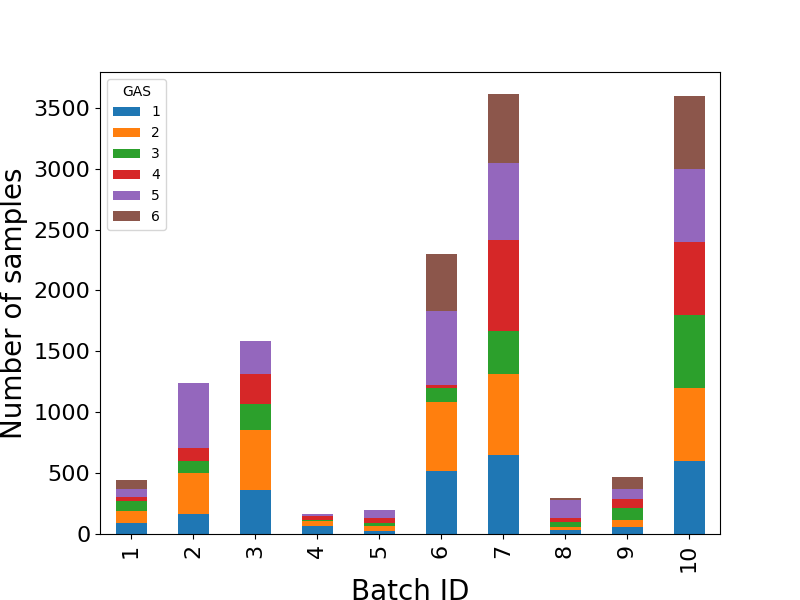
\includegraphics[width=\columnwidth]{../py_imgs/Step0_Count_Batch_Gas.png}
	\caption{Número de muestras de gas por Batch}
	\label{fig: gasBatchCount}
\end{figure}

\begin{figure}[ht!]
	\centering
	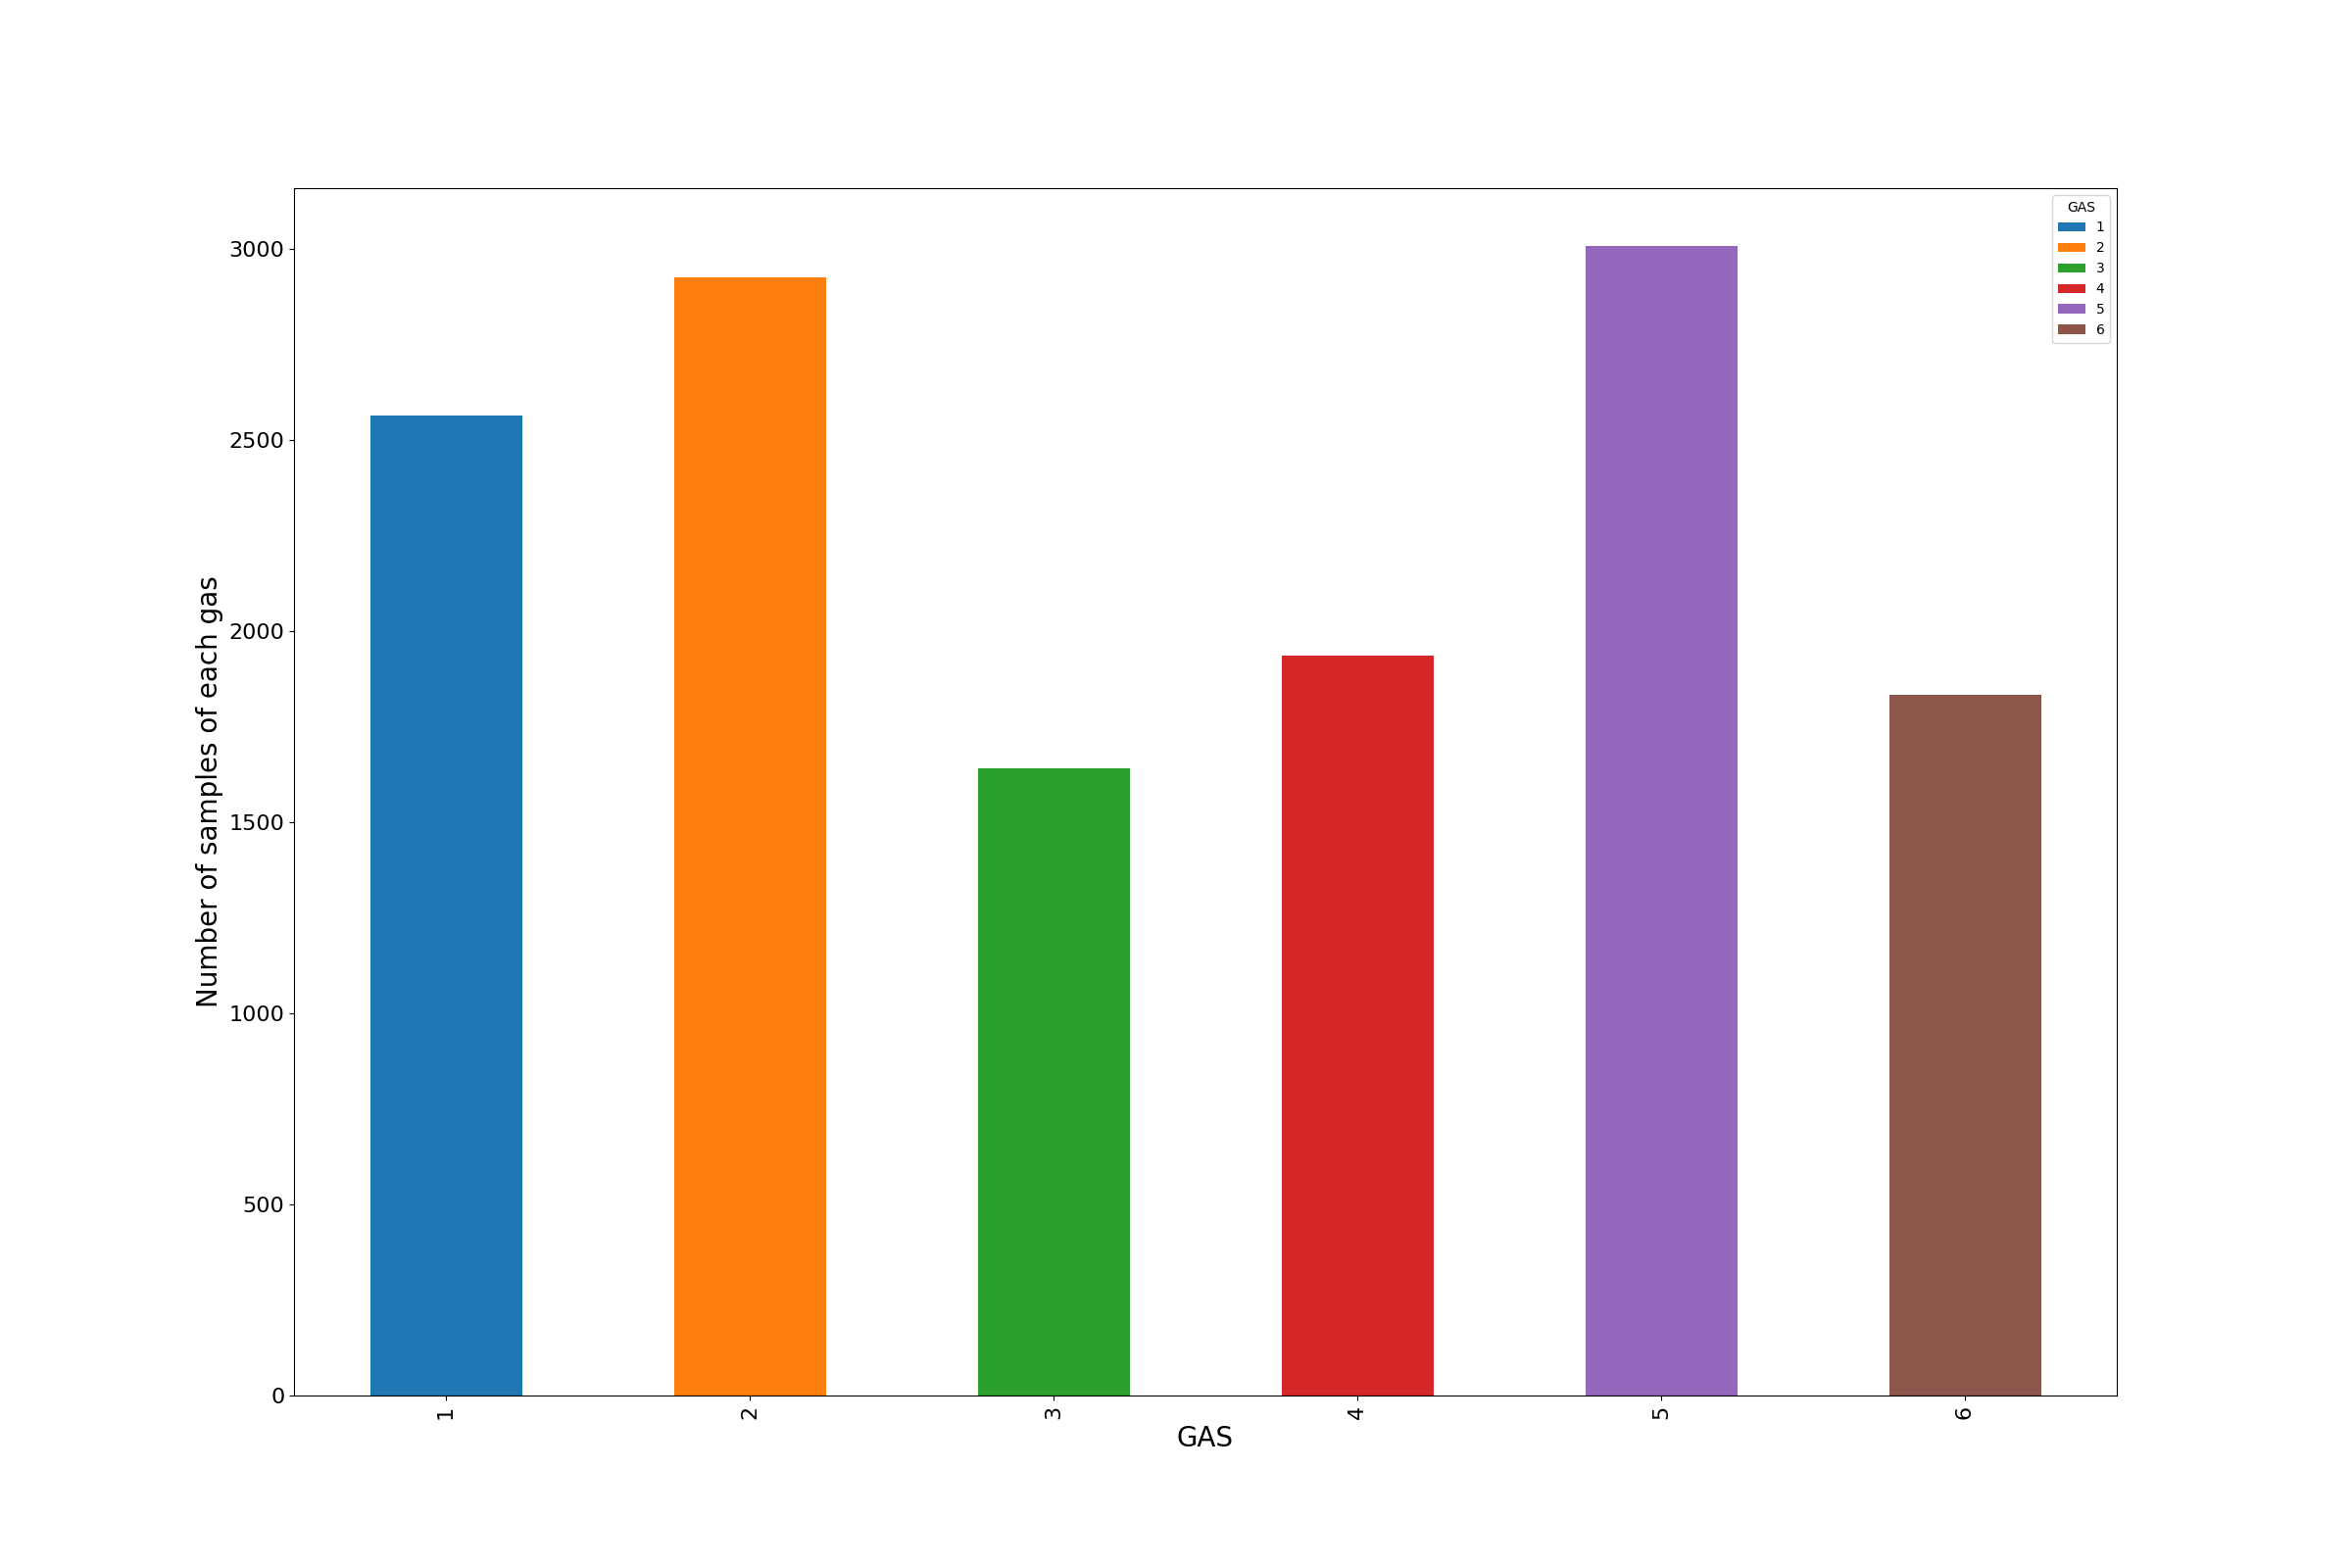
\includegraphics[width=\columnwidth]{../py_imgs/Step0_Count_Gas.png}
	\caption{Número de muestras de cada gas en total}
	\label{fig: gasCount}
\end{figure}

Si observamos los rangos de concentración para cada gas, han sido también diferentes.

\begin{table}
    \centering
    \begin{tabular}{|l|l|l|l|l|l|}
    \hline
    GAS & Minimo & Máximo & Media  & StdDesv \\ \hline
        1 & 2.5 & 600    & 114.95 & 86.64          \\ \hline
        2 & 2.5 & 300    & 116.1  & 79.89          \\ \hline
        3 & 2.5 & 1000   & 323.55 & 272.02         \\ \hline
        4 & 2.5 & 300    & 126.32 & 76.71          \\ \hline
        5 & 10  & 1000   & 228.57 & 217.38         \\ \hline
        6 & 1   & 230    & 47.66  & 32.58          \\ \hline
    \end{tabular}
\end{table}

Esta información es necesario tenerla en cuenta a la hora de entrenar nuestro modelo, ya que
si el rango de variación de los datos es dispar, será recomendable normalizar.




